\documentclass[12pt]{article}

\usepackage[slovene]{babel}
\usepackage[top=1in, bottom=1in, left=1in, right=1in]{geometry}
\usepackage{graphicx}
\usepackage{caption}
\usepackage[hidelinks,unicode]{hyperref}
\usepackage{tikz}
\usepackage{tikz-timing}
\usepackage{amsmath}
\usepackage[utf8]{inputenc}
\renewcommand{\contentsname}{Kazalo}
\renewcommand\listfigurename{Kazalo slik}
\renewcommand{\figurename}{Slika}
\usepackage{listingsutf8}

\begin{document}
\pagenumbering{gobble}
\linespread{1.25}
\begin{titlepage}
  \begin{center}
    
\includegraphics[height=2cm]{slike/vegova.png}\\
    \Huge
    \vspace*{6cm}
    Raziskovanje mej RISCa\\
    \Large
    (računalništvo in informatika)\\
    Raziskovalna naloga\\
  \end{center}
  \vspace{8cm}
  \begin{tabular}{rl}
    Avtor: & Adrian Sebastian Šiška\\
    Mentor: & Aleš Volčini
  \end{tabular}
  \vspace{1cm}
  \begin{center}
    Ljubljana, marec 2022
  \end{center}
\end{titlepage}

\pagebreak
\pagenumbering{arabic}

\tableofcontents

\pagebreak

\listoffigures

\pagebreak

\section{Zahvala}

Zahvaljujem se vsem, ki so mi pomagali pri raziskovanju in pisanju.
Še posebej se zahvaljujem mentorju Alešu Volčiniju za podporo in potrpežljivost.
Pomagla sta mi tudi moja prijatelja Anton Luka Šijanec in Oliver Wagner pri iskanju mojih hroščev.

\pagebreak

\section{Povzetek}
% Da sem ta
\pagebreak

%% ANG ONLY DEU
% \section{Abstract}

\section{Uvod}
% TODO
V raziskovalni nalogi sem si zadal kot cilj izdelavo minimalistične arhitekture.

\subsection{Hipoteza}
V tej nalogi bom preveril resničnost sledeče hipoteze:
\begin{itemize}
  \item Moja lahkotna arhitektura imenovana PUHI je Turing complete.
\end{itemize}

\section{Moja arhitektura}
\begin{figure}[h]
  \centering
  \includegraphics[width=.5\linewidth]{slike/arhitektura.gv.pdf}
  \captionof{figure}{Shematika PUHIja}
\end{figure}
Imenuje se \textit{Praktična URISC hardware implementacija} oz.\ kratica PUHI.\@
\subsection{Kaj je URISC?}
% URGENTLY religate interesting stuff to the compiler
Kratica URISC pomeni \textit{ultimate reduced instruction set computer}, kar bi lahko v slovenščino prevedli kot \textit{računalnik z dokončno zmanjšano množico operacij}.
RISC arhitekture so v praksi, odkar pomnilnik ni več drag, boljše od CISC arhitektur, to nam dokazujejo moderni pametni telefoni, saj skoraj vsi delujejo na arm čipih.
To nam dokaže tudi najpopularnejši ustvarjalec CISC procesorjev, Intel, saj so dandanes njihovi procesorji interno zgrajeni iz tolmača in manjšega RISC procesorja.
Da arhitkturo označimo kot URISC, pa rabimo iti še en korak dajle, in sicer, se znebiti vsek ukazov razen enega.
Zanimiva posedica tega je dejstvo, da lahko ko pišemo strojno kodo popolnoma spustimo polje z instructijo, ostanejo le še njeni argumenti.

V virih najdemo primere, ukazov, ki so sami posebi turing complete, npr.\ x86 mov ukaz.
Jaz sem se raje odločil za 2 instrukciji, ker se njuni rabi ne prekrivata zelo dosti, saj med drugim tudo operirata na različnih magnitudah količine podatkov, je posledica tega dodatka le lažje pisanje programov.
Odločil sem se, da mi je težavnost pisanja programov brez prevajalnika pomembna, ker bi sicer ta naloga vzela še dosti več časa, če bi rabil napisati še prevajalnik.

\subsection{Instrukcije}
Obe instrukciji prejmeta 2 naslova iz rama\footnote{naslov ni nujno povezan z ramom, glej copy instrukcijo} in en meta bit.
V moji izvedbi sem se odločil za 7 bitne\footnote{Ta izbira je arbitrarna, arhitektura podpira n bitne naslove. Tega sem izbral ker je posledična dolžina ukaza v bitni kodi potenca števila 2.} ram naslove.
Za pridobivanje bitnega zapisa preprosto napišemo 1.\ naslov, 2.\ naslov, cifro zeljene instrukcije in meta bit.
Meta bit je nastal zaradi poravnave dolzine ukaza na 2 byta, kar je naredilo pisanje zbirnika in razbirnika nekoliko lažje.
Obe instrukciji se obnasata po principu, da vzameta podatke iz 1.\ naslova in rezultat shranita na 2.\ naslov.

\subsubsection{Instrukcija ``c16''}
To je 1.\ instrukcija oznacena z 0 v binarni obliki.
Njena notacija izhaja iz daljšega imena \textit{copy 16 bits}
Deluje tako, da od njenega 1.\ podanega naslova in še zaporedno nasledjih 15 registrov prekopira v začasen pomnilnik, potem pa jih prekopira na 2.\ naslov in na zaporednih 15 registrov za njim.
Odločitev da bo to 1.\ instrukcija izhaja iz tega, da so same ničle v programu interpretirane kot ukaz brez posledic, kar je uporabno predvsem, ko rabim kaj poravnati na naslov, ki je par mest nižji.
Na začetku je bila zasnovana kot skoraj jump instrukcija, saj z NAND-om ni mogoče vseh bitov v programskem števcu hkrati spremeniti na željeno vrednost.
Posledica spremembe enega pa po enega bita, bi bil skok takoj po 1.\ spremembi saj kontrolna enota vedno preveri števec pred nalaganjem nove instrukcije.

Ko sem kasneje dodal še meta bit, sem se odločil da se bo kopiranje zgodilo iz programskega spomina.
Zaradi tega je nalaganje konstant, kot so nizi ali pa naslovi funkcij postali zelo preprosti in hitri.
Limitacija tega je, da sem uporabil 7 bitni naslov za pridobivanje podatkov iz pomnilnika opisanega z 16 biti.
Zaradi tega večina pomnilnika še vedno ni na voljo, kot rešitev temu pa sem se odločil, da sem uporabil skrite registre kot nastavitev strani programskega pomnilnika.

Skriti biti nastanejo kot stranski učinek slabe definicije zaporednih registrov.
Kaj se zgodi če nekaj skopiramo na zadnji register?
Zdi se mi da je najbolj uporaben odgovor, da rečem da so za ``zadnjim registrom'' še skriti registri.
Do njihove vsebine se da dostopati le z c16 ukazom, kar se mi ne zdi problem, saj menim, da bo ta konfiguracija redko spremenjena čez potek programa.

Torej se ukaz \verb|c16 0x22, 0x44, 0| prevede v \verb|0100010 1000100 0 0|, kar bi lahko predstavili z Cejevsko vrtico kode\\
\verb|int *a=0x22; int* b=0x44; *b=*a;*(b+1)=*(a+1)|\ldots \verb|*(b+15)=*(a+15)|.

\subsubsection{Instrukcija ``Nox''}
To je 2.\ instrukcija oznacena z 1 v binarni obliki.
Ime izhaja iz njenega kratkega opisa: \textit{Nanad or XOR}.
Najprej sem probal uporabiti le XOR, kot edini ukaz za minpulacijo bitov, vendar sem hitro ugotovil, da se iz samo XORa ne da rekonstuirati vseh ostalih logičnih vrat.
Zato sem se odločil še za naj pogosteje izbrana univerzalna vrata NAND.\@

Ta so s seboj privlekla nove probleme kot npr.\ pogojni skoki naprej so postali zelo dragi.
Programski števec bi lahko bil viden samo c16 ukazu, vendar bi to preprečilo relativne skoke, kjer spremenim le 1 bit v njem.
Pogojni relativni skoki so nadaljevanje tega. Ker vem kje se nahaja trenuten ukaz, lahko vem v kakšnem stanju je nek bit v programskem števcu.
S kombiniranjem enice v programskem števcu in nekega podatka v ramu lahko skočim nazaj, samo če je tudi podatek v ramu enica.
Pogojen skok naprej ni izvedljiv na tak način. Saj bo na enobitnem mesu, če ga želimo povečati morala biti ničla.
NAND pravi, da če je kateri koli izmed argumentov 0, da bo rezultat vedno 1, kar pomeni da naš \textit{pogoj} ni bil upoštevan.

Zaradi dragih skokov in lahke ponastavitve celice na 0, sem se odločil da dodam še XOR.\@
Par vrat sem kombiniral v 1 instrukcijo, kjer meta bit izbira med njima.

\begin{displaymath}
  f(A,B,M) =
  \begin{cases}
    NAND(*A\footnote{*N pomeni priklic iz rama z naslovom N}, *B) \rightarrow *B & M=0\\
    XOR(*A, *B) \rightarrow *B & M=1
  \end{cases}
\end{displaymath}
Oz.\ zapisano v logični notaciji.
\begin{displaymath}
  \overline{(AB)}(A+B+\overline{C})
\end{displaymath}

Torej se ukaz \verb|Nox 0x15, 0x53, 0| prevede v \verb|0010101 1010011 1 0|, kar bi lahko predstavili z Cejevsko vrtico kode \verb|int *a=0x15;int *b=0x53;*b=NAND(*a,*b)|.

\subsection{Enobitni registri}
% vsi registri so eneaki, samo eni so bol enaki
Kot ram sem si zamislil \textit{trak} enobitnih registrov.
Zaradi preprostosti, je programski števec preslikan čez prvih 16 registrov, da lahko tudi ukaz Nox z njem operira.
Ves I/O je tudi preslikan na registre, in sicer na prve štirji za števcem.
Število vseh registrov je funkcija dolžine naslova rama in velikosti programskega števca.
Velikost programskega števca je potrebno upoštevati, saj je glede na njega definiran ukaz za kopiranje, in polsedica ukaza za kopirajne so skriti registri.
Za računanje dolžine traka registrov sem pripravil preprosto formulo.
$F(N,P)$, v mojem primeru $F(7,16)$, zračuna število registrov, ki jih imam na razpolago, pri danem N in P.
\begin{center}
  \begin{displaymath}
    F(N,P)=2^{N}+P-1
  \end{displaymath}
  $F(N,P)$ je število registrov, $N$ je dolžina binarnega naslova, $P$ je programski števec
\end{center}

\subsection{Komunikacija z zunanjim svetom}
Za izvedbo vhodno-izhodnih operacij, sem se odločil da bom implementiral svojo 4 žično komunikacijo.
Ta lahko asinhrono bere informacije po bitih.
Asinhronost je pomembna lastnost, saj nimam nikjer prostora da bi dodal začasen pomnilnik, ki bi shranjeval podatke, preden bi procesor imel čas, da se začne ukvarjati z njimi.
Interrupt tudi ni dobro nadomestilo asinhronosti, saj bi dodal ogromno kompleksnosti, kot npr.\ najmanj 16 dodatnih registrov, instrukcijo za branje z njih in možnost spreminjanja registrov, ki ni posledica nekega ukaza.
Lepa lastnost štirižičnega protokola je tudi, da se dve napravi z lahkoto skupaj poveže, saj moramo le izhode iz ene priklopti v vhode druge.
\begin{center}
  \begin{tabular}{ccc}
    $A_{OUT}  $ & \texttiming{LHHHLLLLLL} & $B_{IN}$\\
    $A_{OUT_A}$ & \texttiming{LLHZLLLLLL} & $B_{IN_A}$\\
    $A_{IN}   $ & \texttiming{LLLLLHHHHL} & $B_{OUT}$\\
    $A_{IN_A} $ & \texttiming{LLLLLLHZLL} & $B_{OUT_A}$
  \end{tabular}\footnote{modra črta na sredini prikaže stanje, kjer ena naprava drži signal pri logični enici, druga naprava pa ga proba nastaviti na ničlo}

  \text{Primer pošiljanja enice od A do B in od B do A}
\end{center}
Za pošiljanje informacij najprej počakaš da je $OUT_{A}$ dovoljen, torej 0.
Nato lahko pišemo kar hočemo v $OUT$, dokler ne želimo vrednosti \textit{oddati}, kar naredimo s tem da napišemo enico na $OUT_{A}$.

Za prejemanje informacij je podoben postopek.
Začnemo z Preverjanjem $IN_{A}$, kot da bi gledali nabiralnik, če nam je poštar kaj prinesel.
Čim dobimo napisano enico, smemo interpretirati karkoli je v $IN$, kot podatke.
Da dobimo naslednji znak, priklopimo pulldown upor na $IN_{A}$.
To druga naprava zazna in čimprej spusti $IN_{A}$ na 0.


\section{Izdelava} %TODO
Za uspešno izdelavo sem se odločil da bom potreboval okolje, kjer lahko testiram spremembae arhitekture in mojie programe.
Zato sem se lotil pisanja virtualnega stroja, ker pa je teško vedeti če zares deluje, sem začel delo na zbirniku, da ne bi več rabil na roke pisati enk in ničel.
Seveda je izdelava zbirnika tudi težka, zato sem razvil še razbirnik, da preverim delovanjei zbirnika.
Izdelava le tega je bila nekoliko lažja, kljub temu sem čez nekaj dni našel večjo napako pri de šifriranju ukazov.

\subsection{Zbirnik (assembler)}
Najprej celotno datoteko podamo NASM-ovem prepreprocesorju.
Potem za vsako vrstico v datoteki:
\begin{itemize}
  \item preiščemo vrstico za par ``$<py>$'' simbolov, ki tvorita python blok.
  Vsaka uporabnikova konstanta je tako ali tako interpretirana skozi oči pythona, vendar nastane problem, ko probamo interpretirati pythonov izraz ki vsebuje vejice.
  Vejice so namreč ločilo med polji zato moj preprost razpoznavalnik nepravilno nareže en pythonov izraz na več majhnih delov, ki sami po sebi nehajo biti veljavni.
  \item Ko končamo in vse py bloke zamenjamo z njigovimi zračunanimi vrednostmi v vrstici.
  \item Nato klasificiramo vsako vrsico v eno izmed 5 možnih vrst.
  \begin{itemize}
    \item Komentar ali prazna vrstica, ki jih lahko varno spustimo,
    \item Surovi binarni podatki, ki jih direktno zapišemo v datoteko,
    \item Premik v programu, premaknemo mesto pisanja in nadaljujemo,
    \item Instrukcija v procesorju, ki jo dešifriramo, izračunamo njene argumente in zapišemo,
    \item Naslov, katerega pozicijo si zapomnimo, da bomo kasneje lahko omenjali predmet pred katerim stoji.
  \end{itemize}
\end{itemize}

\subsubsection{Preprocessor}
Preprocessor skrbi za dodajanje večih datotek skupaj in dešifriranje makrotov ter definicij.
Nasm je precej popularen assembler, ki mi dovoli, da zlahkoto pokličem le njegov preprocesor.
Bolj primeren je kot c-jev preprocesor, ker zaradi formata zbornika, ne smemo zanemariti novih vrstic.
\subsubsection{Razbirnik (Dissasembler)}
\begin{center}
  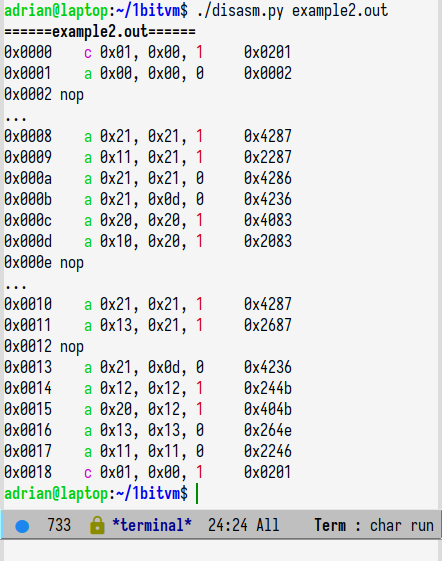
\includegraphics[width=.3\linewidth]{slike/razbirnik.png}
  \captionof{figure}{Primer uporabe razbirnika}
\end{center}
Seveda je bilo nekaj problemov na katere sem naletel med potjo do zbirnika.
Zato sem z malo pomoči Oliverja napisal še manjši program, ki se sprehodi čez datoteko in jo interpretira v instrukcije in njene argumente.
Izpiše nam naslov na katerem se ukaz nahaja, ukaz sam, meta bit in še šestnajstiški prikaz tega ukaza, saj ne loči med podatki in ukazi.

\subsubsection{Iskanje ukazov s surovo silo}
Pisanje makrotov, kot so add je človeku zelo težko opravilo.
Seveda se da najti kombinacijo NAND-ov in xorov, ki bi mi vrnila seštevek dveh cifer, vendar ne morem biti prepričan, da je to najhitrejši algoritem za to.
Zato sem napisal program, ki to piše namesto mene.
Ideja je v tem, da za vsak možen vhod v N celic poiskusimo vse možne ukaze, in gledamo, kdaj dobimo nov rezultat.
Ko dobimo kaj novega, lahko preprosto ponovimo postopek.
Iz tega lahko generiramo tabelo rezultatov glede na vse možne vhode.

Prva implementacija tega programa je bila napisana v pythonu in bi po mojih ocenah trajalo nekaj tednov, da bi dobil popolno tabelo vseh možnih rezultatov.
Zato sem prepisal cel program v C, in z uporabo večih niti, skrajšal čas iskanja na 3 sekunde.

\section{Virtualna implementacija}
Da zares lahko pokažem delovanje naprave, moram nekako prikazati kako deluje, in to na najlažji način dosežem z implementacijo v virtualnem okolju.
Zato sem se lotil pisanja virtualne naprave v pitonu.
Svoji 2 izhodni žici ima povezani na standardni izhod, svoji 2 vhodni žici pa na standardni vhod.
Tako lahko preko terminala komuniciramo z virtualno napravo.
To lahko najlažje vidimo v 1.\ primeru, kjer naprava izpiše ``Živjo'', ali v 2.\ primeru, kjer nam naprava vrne nazaj vsak bit, ki ga prejme.
\subsection{cellular automata}
\begin{center}
  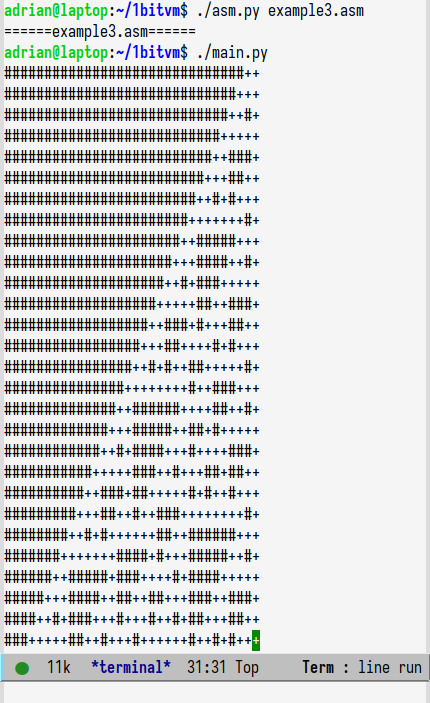
\includegraphics[width=.3\linewidth]{slike/pravilo110.png}
  \captionof{figure}{Prikaz delovanja celičnega avtomata na PUHI arhitekturi.}
\end{center}
Kot metodo dokazovanja, da je PUHI turing complete, sem izbral emulacijo drugega turing complete sistema.
Eden izmed najbolj preprostih, čeprav še vedno dovolj kompleksnih, da je univerzalen, je Celični avtomat z pravilom 110.
Seveda ne morem implementirati neskončno dolgega enodimenzionalnega traka, na katerem bi simuliral izvajanje tega pravila, lahko pa pokažem, da bi se to dalo implementirati, če bi moja naprava imela neskončno rama.

\section{Zaključek}
\subsection{Hipoteza}
\begin{itemize}
  \item Moja lahkotna arhitektura imenovana PUHI je Turing complete.
  Hipoteza potrjena, saj lahko popolnoma emulira sistem, za katerega je že bilo dokazano, da je turing complete
\end{itemize}

\section{Nadaljne raziskave}
Zdi se mi pomembno omeniti, da lahko med tem ko ohranimo preprostost dizajna moje eno-bitne arhitekture, močno razširimo njeno moč, s tem da jo postavimo kot generator programskega spomina sebe.

\section{Priloge}

\lstset{
  basicstyle=\footnotesize,
  breaklines=true,
  frame=single,
  stepnumber=5,
}
\lstdefinestyle{py}{
  language=Python,
}

\lstdefinestyle{asm}{
  language=[x86masm]Assembler,
  morekeywords={copy, nand, xor, x, a, c},
}
\lstdefinestyle{cst}{
  language=C,
}

\lstinputlisting[style=py,caption=asm.py]{1bitvm/asm.py}
\lstinputlisting[style=py,caption=disasm.py]{1bitvm/disasm.py}
\lstinputlisting[style=asm,caption=example.asm]{1bitvm/example.asm}
\lstinputlisting[style=asm,caption=example2.asm]{1bitvm/example2.asm}
\lstinputlisting[style=asm,caption=example3.asm]{1bitvm/example3.asm}
\lstinputlisting[style=asm,caption=std.asm]{1bitvm/std.asm}
\lstinputlisting[style=py,caption=main.py]{1bitvm/main.py}
%\lstinputlisting[caption=Primer razporeditve pomnilnika]{1bitvm/mem}
\lstinputlisting[style=py,caption=oneb\_vm.py]{1bitvm/main.py}
\lstinputlisting[style=cst,caption=program za poskušanje vseh logičnih vrat]{gate-bf/main.c}




\pagebreak
\section{Viri in literatura}
$[1]$ dosegljivo: \url{https://uops.info/} [23.3.2022]\\
$[2]$ dosegljivo: \url{https://cs.stanford.edu/people/eroberts/courses/soco/projects/risc/risccisc/} [23.3.2022]\\
$[3]$ dosegljivo: \url{https://wpmedia.wolfram.com/uploads/sites/13/2018/02/15-1-1.pdf} [23.3.2022]\\
$[4]$ Modrost mojega prijatelja Oliverja Wagnerja.\ dosegljivo: \url{https://github.com/Oliwerix}\\

% \pagebreak
% \section{Viri slik}
\end{document}
